\section{}

\textbf{Tiempo de lectura:} \{s09-reading-time\}

Los primeros sistemas informáticos solo permitían que un programa se
ejecutase cada vez. Dicho programa tenía control completo sobre el
sistema y acceso a todos los recursos del mismo. Por el contrario, los
sistemas \textbf{multitarea} actuales permiten que múltiples programas
sean cargados y ejecutados concurrentemente.

Obviamente esta evolución implica un control más fino y la
compartimentación de los diversos programas, para que no interfieran
unos con otros. Esto, a su vez, conduce a la aparición de la noción de
\textbf{{}proceso}, que no es sino la unidad de trabajo en un sistema
operativo moderno de tiempo compartido.

Por simplicidad, en este capítulo utilizaremos los términos
\textbf{trabajo} y \textbf{proceso} de forma indistinta. A fin de
cuentas tanto los \textbf{trabajos} en los antiguos \emph{mainframes}
como los \textbf{procesos} en los sistemas modernos son la unidad de
trabajo en sus respectivos sistemas y el origen de toda actividad en la
CPU.

Por último, antes de continuar, es importante señalar que en un sistema
operativo hay varios tipos de procesos:

\begin{itemize}
\item
  \textbf{Procesos del sistema}{}. Ejecutan el código del sistema
  operativo contenido en los \textbf{programas del sistema}, que
  generalmente sirven para hacer tareas del sistema operativo que es
  mejor mantener fuera del núcleo.
\item
  \textbf{Procesos de usuario}{}. Ejecutan el código contenido en los
  \emph{programas de aplicación}.
\end{itemize}

Sin embargo, en lo que resta de capítulo, no estableceremos ninguna
distinción entre ellos. En lo que respecta a la gestión de estos
procesos en el sistema, no hay ninguna diferencia.

\section{El proceso}\label{_el_proceso}

Como ya hemos comentado con anterioridad, un \textbf{{}proceso} es un
programa en ejecución (véase el
\hyperref[sect-componente-gestion-de-procesos]{???} para una
definición más completa). Sin embargo, los procesos no solo están
compuestos por el código del programa, sino que también son importantes
otros elementos:

\begin{description}
\item[Segmento de código{}]
Contiene las instrucciones ejecutables del programa. También es conocido
como segmento \textbf{text}{} o \textbf{.text}.
\item[Segmento de datos{}]
Contiene las variables globales y estáticas del programa que se
inicializan con un valor predefinido. También es conocido como segmento
\textbf{.data}.
\item[Segmento BSS{}]
El segmento BSS ---siglas de \emph{block started by symbol}--- contiene
las variables globales y estáticas del programa inicializadas a 0 o sin
inicialización explícita. Como contiene variables globales sin valor
inicial, en el ejecutable, generalmente, solo se guarda la longitud que
debe tener este segmento en la memoria. También es conocido como
segmento \textbf{.bss}.

En el esquema de la \hyperref[fig-proceso-en-memoria]{Anatomía de un
proceso en memoria.}, este segmento suele ir junto al de datos.
\item[Pila{}]
Contiene datos temporales, como los parámetros y direcciones de retorno
de las funciones y las variables locales.
\item[Montón{}]
Contiene el espacio de la memoria que se asigna dinámicamente durante la
ejecución del proceso. También es conocido como \textbf{{}heap}.
\item[Información sobre el estado actual de ejecución]
Como el \textbf{contador de programa}, los valores de los
\textbf{registros de la CPU}, el \textbf{estado} del proceso y más
(véase el \hyperref[_bloque_de_control_de_proceso]{Bloque de control de
proceso}).
\end{description}

Los \textbf{segmentos de código}, \textbf{datos} y \textbf{BSS} por lo
general son secciones dentro del archivo ejecutable que contiene el
programa. El resto de elementos los crea el sistema operativo al cargar
el programa y crear el proceso.

Como vimos en el \hyperref[sect-componente-gestion-de-procesos]{???}
varios procesos pueden estar asociados al mismo programa, pero no por
eso dejan de ser distintos procesos. Todos tendrán una copia del mismo
segmento de código, pero diferente: contador de programa, valores en los
registros de la CPU, pila, segmento de datos, montón y demas
propiedades.

En la \hyperref[fig-proceso-en-memoria]{Anatomía de un proceso en
memoria.} se puede observar la disposición de algunos de estos elementos
de un proceso en el espacio de usuario en la memoria.

\begin{figure}
\centering
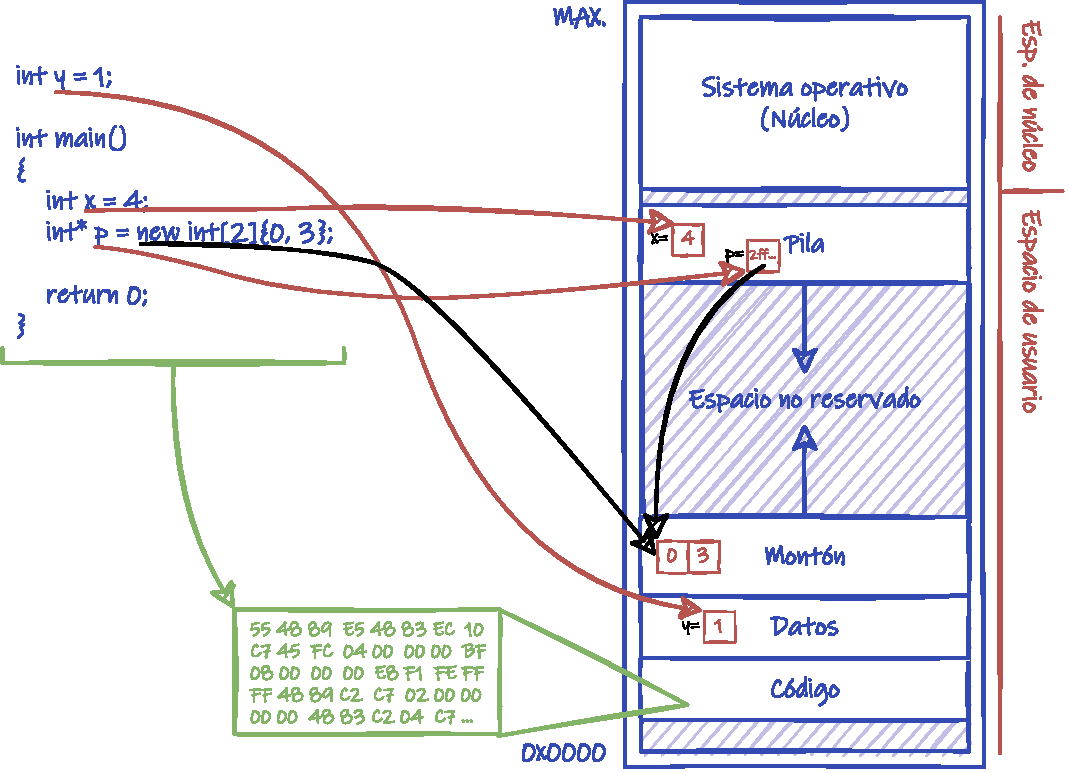
\includegraphics[width=0.8\textwidth]{media/C09_procesos/proceso_en_memoria.pdf}
\caption{Anatomía de un proceso en
memoria.}\label{fig-proceso-en-memoria}
\end{figure}

\section{Estados de los procesos}\label{_estados_de_los_procesos}

Cada proceso tiene un \textbf{estado} que cambia a lo largo de su
ejecución y que está definido, parcialmente, por la actividad que
realiza actualmente el propio proceso.

\begin{figure}
\centering
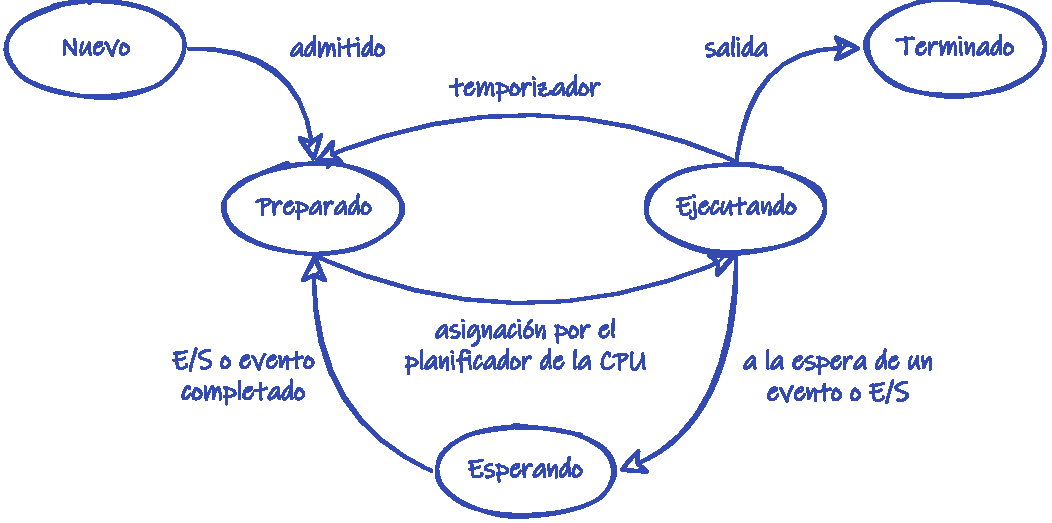
\includegraphics[width=0.8\textwidth]{media/C09_procesos/diagrama_estado_proceso.pdf}
\caption{Diagrama de estado de un
proceso.}\label{fig-diagrama-estado-proceso}
\end{figure}

Los estados por los que puede pasar un proceso varían de un sistema
operativo a otro, aunque los siguientes son comunes a todos ellos:

\begin{description}
\item[Nuevo]
El proceso está en proceso de creación. Este estado existe porque la
creación de un proceso no es algo instantáneo. Necesita de varias
operaciones que pueden tardar tiempo en realizarse, como: reservar
memoria libre, cargar el programa en la memoria, inicializar estructuras
de datos y configurar el entorno de ejecución.
\item[Ejecutando]
El proceso está siendo ejecutado en la CPU. Para eso tiene que haber
sido escogido por el planificador de la CPU de entre todos los procesos
en estado \textbf{preparado}. Solo puede haber un proceso en este estado
por CPU en el sistema.
\item[Esperando]
El proceso está esperando por algún \textbf{evento} como, por ejemplo,
que termine una operación de E/S solicitada previamente o que otro
proceso termine su ejecución. Múltiples procesos pueden estar en este
estado de espera.
\item[Preparado]
El proceso está esperando a poder usar la CPU. Múltiples procesos pueden
estar en este estado.
\item[Terminado]
El proceso ha finalizado su ejecución y espera a que el sistema
operativo recupere los recursos que le fueron asignados. Como en el caso
del estado \textbf{nuevo}, este estado existe porque terminar un proceso
no es algo instantáneo.
\end{description}

El diagrama de estados de los procesos, con las transiciones posibles
entre ellos, se muestra en la
\hyperref[fig-diagrama-estado-proceso]{Diagrama de estado de un
proceso.}.

\section{Bloque de control de
proceso}\label{_bloque_de_control_de_proceso}

{} El \textbf{bloque de control de proceso} o \textbf{{}PCB}
(\emph{Process Control Block}) es una estructura de datos que representa
a cada proceso en el sistema operativo y que guarda información sobre su
estado de actividad actual.

En el sistema hay un PCB por proceso y sirve de almacén para cualquier
información que puede variar de un proceso a otro:

\begin{itemize}
\item
  \textbf{Estado del proceso}. El estado actual del proceso de la lista
  que hemos visto anteriormente. Por ejemplo: nuevo, preparado,
  esperando, etc.
\item
  \textbf{Contador de programa}. Indica la dirección de la próxima
  instrucción del proceso que debe ser ejecutada por la CPU. Obviamente,
  durante el estado \textbf{ejecutando} el contador de programa está en
  el registro correspondiente de la CPU. Su valor se guarda en el PCB al
  salir el proceso de la CPU para que comience ejecutarse en ella otro
  proceso.
\item
  \textbf{Registros de la CPU}. El valor de los registros de la CPU
  también forman parte del estado de actividad del proceso. Como en el
  caso del \textbf{contador de programa}, durante el estado
  \textbf{ejecutando} los valores están en los registros de la CPU, pero
  se guardan en el PCB cuando el proceso sale de la CPU para que se
  ejecute otro proceso.
\item
  \textbf{Información de planificación de la CPU}. Incluye la
  información requerida por el planificador de la CPU. Por ejemplo la
  prioridad del proceso, punteros a las colas de planificación donde
  está el proceso, punteros al PCB del proceso padre y de los procesos
  hijos, etc.
\item
  \textbf{Información de gestión de la memoria}. Incluye la información
  requerida para la gestión de la memoria. Por ejemplo los valores de
  los registros base y límite que definen el área de la memoria física
  que ocupa el proceso ---en el caso de se use asignación contigua de
  memoria (véase el \hyperref[_asignacion_contigua_de_memoria]{???} o
  la dirección a la tabla de páginas ---en el caso de que se use
  paginación (véase el \hyperref[paginacion]{???})---.
\item
  \textbf{Información de registro}. Aquí se incluye la cantidad de CPU
  usada, límites de tiempo en el uso de la CPU, estadísticas de la
  cuenta del usuario a la que pertenece el proceso, estadísticas de la
  ejecución del proceso, etc.
\item
  \textbf{Información de estado de la E/S}. Incluye la lista de
  dispositivos de E/S reservados por el proceso, la lista de archivos
  abiertos, etc.
\end{itemize}

\section{Colas de planificación}\label{_colas_de_planificacion}

{} En los sistemas operativos hay diferentes \textbf{colas de
planificación} para los procesos en distintos \textbf{estados}.

\begin{description}
\item[Cola de trabajo{}]
Contiene todos los trabajos en el sistema, de manera que cuando entran
en el sistema van a esta cola, a la espera de ser escogidos para ser
cargados en la memoria y ejecutados. Esta cola existía en los
\textbf{sistemas multiprogramados}, pero no existe en los
\textbf{sistemas de tiempo compartido} ni en los sistemas operativos
modernos posteriores.
\item[Cola de preparados{}]
Contiene a los procesos que están en estado \textbf{preparado}. Es
decir, procesos cargados en la memoria principal que esperan para usar
la CPU. La cola de preparados es generalmente una lista enlazada de PCB,
donde cada uno incluye un puntero al PCB del siguiente proceso en la
cola.
\item[Colas de espera{}]
Contienen a los procesos que están en estado \textbf{esperando}. Es
decir, que esperan por un evento concreto, como por ejemplo la
finalización de una petición de E/S. Estas colas también suelen ser
implementadas como listas enlazadas de PCB y suele haber una por evento,
de manera que cuando ocurre algún evento todos los procesos en la cola
asociada pasan automáticamente al estado \textbf{preparado} y a la
\textbf{cola de preparados}.
\item[Colas de dispositivo{}]
Son un caso particular de cola de espera. Cada dispositivo de E/S tiene
asociada una \textbf{cola de dispositivo} que contiene los procesos que
están \textbf{esperando} por ese dispositivo en particular.
\end{description}

Una manera habitual de representar la planificación de procesos es a
través de un diagrama de colas como el de la
\hyperref[fig-colas-de-planificacion-procesos]{Diagrama de colas de
la planificación de procesos.}.

\begin{figure}
\centering
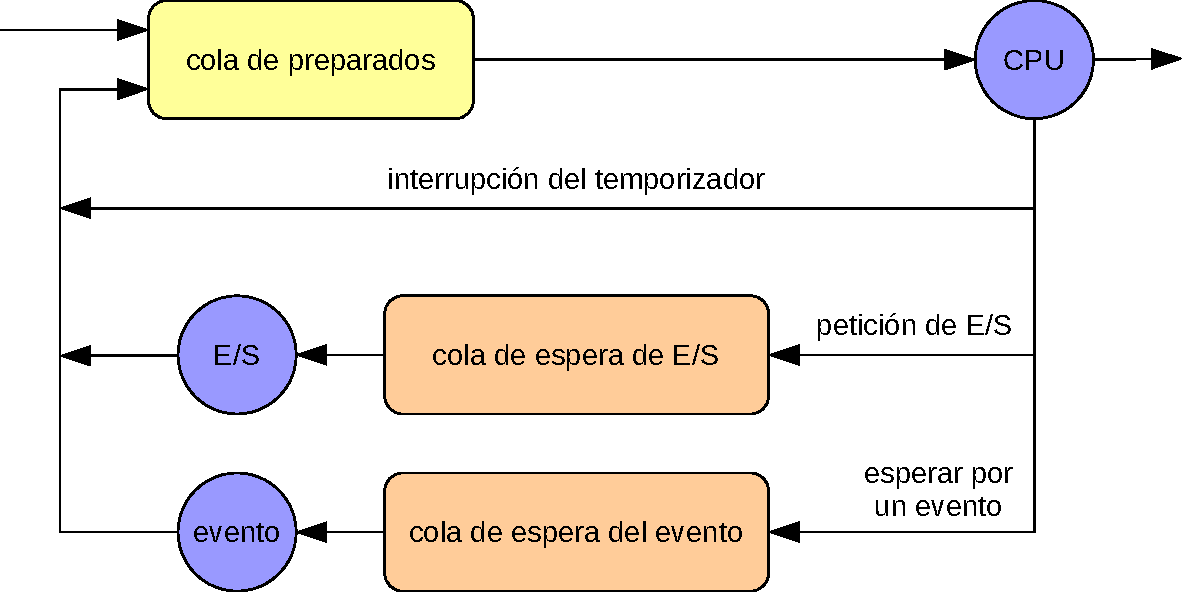
\includegraphics[width=0.8\textwidth]{media/C09_procesos/colas_planificación_procesos.pdf}
\caption{Diagrama de colas de la planificación de
procesos.}\label{fig-colas-de-planificacion-procesos}
\end{figure}

Analizándolo podemos tener una idea clara del flujo típico de los
procesos dentro del sistema:

\begin{enumerate}
\def\labelenumi{\arabic{enumi}.}
\item
  \textbf{Un nuevo proceso llega al sistema}. Una vez pasa del estado
  \textbf{nuevo} a \textbf{preparado} es colocado en la \textbf{cola de
  preparados}. Allí espera hasta que es seleccionado por el
  \textbf{planificado de la CPU} para su ejecución y se le asigna la
  CPU. Mientras se ejecuta pueden ocurrir varias cosas:

  \begin{itemize}
  \item
    \textbf{El proceso solicita una operación de E/S} por lo que
    abandona la CPU y es colocado en la \emph{cola de dispositivo}
    correspondiente en estado \textbf{esperando}. No debemos olvidar que
    aunque en nuestro diagrama no exista más que una de estas colas, en
    un sistema operativo real suele haber una para cada dispositivo.
  \item
    \textbf{El proceso puede querer esperar por un evento}. Por ejemplo,
    puede crear otro proceso y esperar a que termine. En ese caso el
    proceso hijo es creado, mientras el proceso padre abandona la CPU y
    es colocado en una \textbf{cola de espera} en estado
    \textbf{esperando} hasta que el proceso hijo termine. La terminación
    del proceso hijo es el evento que espera el proceso padre para salir
    de la \textbf{cola de espera} y entrar en la \textbf{cola de
    preparados} para continuar su ejecución en la CPU cuando sea
    posible.
  \item
    \textbf{El proceso puede ser sacado forzosamente de la CPU}, como
    resultado de la interrupción del temporizador, que permite
    determinar cuando un proceso lleva demasiado tiempo ejecutándose,
    así que es colocado en la \textbf{cola de preparados} en estado
    \textbf{preparado}.
  \end{itemize}
\item
  \textbf{Cuando las esperas concluyen, los procesos vuelven a la cola
  de preparado}, pasando del estado de espera al de preparado.
\item
  \textbf{Los procesos repiten este ciclo hasta que terminan}. En ese
  momento son eliminados de todas las colas mientras el PCB y los
  recursos asignados son recuperados por parte del sistema operativo
  para poder usarlos con otros procesos.
\end{enumerate}

\section{Planificación de procesos}\label{_planificacion_de_procesos}

Durante su ejecución, los procesos se mueven entre las diversas colas de
planificación a criterio del sistema operativo. Este proceso de
selección debe ser realizado por el \textbf{planificador} adecuado:

\begin{itemize}
\item
  El \textbf{planificador de largo plazo}{} o \textbf{planificador de
  trabajos}{}--- selecciona los trabajos desde la \textbf{cola de
  trabajos} en el almacenamiento secundario ---dónde están todos
  almacenados--- y los carga en memoria.

  Este planificador se usaba en los \textbf{sistemas multiprogramados},
  donde había una \textbf{cola de trabajos}. Los \textbf{sistemas de
  tiempo compartido} posteriores y los sistemas operativos modernos,
  carecen de \textbf{planificador de largo plazo}, porque los programas
  se cargan directamente en memoria para ser ejecutados cuando el
  usuario lo solicita.
\item
  El \textbf{planificador de corto plazo}{} o \textbf{planificador de
  CPU}{} selecciona uno de los procesos en la cola de preparados y lo
  asigna a la CPU. Obviamente este planificador es invocado cuando un
  proceso en ejecución abandona la CPU, dejándola disponible para otro
  proceso.
\item
  El \textbf{planificador de medio plazo} {} era utilizado en algunos
  sistemas para sacar procesos de la memoria cuando escasea y
  reintroducirlos posteriormente cuando vuelve a haber suficiente
  memoria libre. A este esquema se le denomina \textbf{{}intercambio}
  ---o \textbf{\emph{{}swapping}}.

  Esto era útil en sistemas antiguos donde un proceso tenía que estar
  cargado completamente en la memoria para poder ejecutarse. Así que si
  faltaba memoria, se podía suspender un proceso completo, preservar el
  contenido de su memoria en disco y liberar la memoria ocupada para
  usarla con otros procesos.

  En los sistemas de propósito general modernos no se utiliza
  \textbf{planificador de medio plazo} porque utilizan técnicas de
  \textbf{memoria virtual} (véase el \hyperref[memoria_virtual]{???}),
  que permite mover parte de la memoria de los procesos al disco para
  liberar memoria, sin tener que suspender la ejecución del proceso.
\end{itemize}

\section{Cambio de contexto}\label{_cambio_de_contexto}

El \textbf{{}cambio de contexto} es la tarea de asignar la CPU a un
proceso distinto al que la tiene asignada en el momento actual. Esto
implica salvar el estado del viejo proceso en su PCB y cargar en la CPU
el estado del nuevo. Entre la información que debe ser preservada en el
PCB se incluyen:

\begin{itemize}
\item
  El \textbf{contador de programa}.
\item
  Los \textbf{registros de la CPU}.
\item
  El \textbf{estado del proceso}.
\item
  La \textbf{información de gestión de la memoria}. Por ejemplo, la
  información necesaria para configurar el espacio de direcciones del
  proceso.
\end{itemize}

El cambio de contexto es sobrecarga pura, puesto que no hace ningún
trabajo útil mientras se conmuta. Su velocidad depende de aspectos tales
como: el número de registros, la velocidad de la memoria y la existencia
de instrucciones especiales.

Algunas CPU disponen de instrucciones especiales para salvar y cargar
todos los registros de manera eficiente. Esto reduce el tiempo que la
CPU está ocupada en los cambios de contexto.

Otra opción es el uso de
\href{https://en.wikipedia.org/wiki/Register_file}{juegos de registros},
como es el caso de los procesadores \{ultrasparc\} e \{itanium\}. Con
ellos el juego de registros actual de la CPU se mapea sobre un banco de
registros mucho más extenso. Al hacer cambio de contexto, se mapea el
juego de registros a otros registros diferentes del banco. Esto permite
a la CPU almacenar de forma eficiente el valor de los registros de más
de un proceso, sin que en cada cambio de contexto sea necesario
copiarlos al PCB del proceso en la memoria principal.

\section{Operaciones sobre los
procesos}\label{_operaciones_sobre_los_procesos}

En general es necesario que los procesos pueden ser creados y eliminados
dinámicamente, por lo que los sistemas operativos deben proporcionar
servicios para la creación y terminación de los mismos.

\subsection{Creación de procesos}\label{_creacion_de_procesos}

Un proceso ---denominado \textbf{padre}--- puede crear múltiples
procesos ---los \textbf{hijos}--- utilizando una llamada al sistema
específica para la creación de procesos. Cada proceso creado se
identifica de manera unívoca mediante un \textbf{{}identificador de
proceso} o \textbf{{}PID} (\emph{Process Identifier}), que normalmente
es un número entero.

Por ejemplo en sistemas POSIX un programa puede crear otro proceso así:

\begin{Shaded}
\begin{Highlighting}[]
\NormalTok{pid\_t pid }\OperatorTok{=}\NormalTok{ fork}\OperatorTok{();}
\end{Highlighting}
\end{Shaded}

mientras que en Windows API es así:

\begin{Shaded}
\begin{Highlighting}[]
\NormalTok{PROCESS\_INFORMATION pi }\OperatorTok{=} \OperatorTok{\{}\DecValTok{0}\OperatorTok{\};}
\ControlFlowTok{if} \OperatorTok{(}\NormalTok{ CreateProcess}\OperatorTok{(} \StringTok{"C:}\SpecialCharTok{\textbackslash{}\textbackslash{}}\StringTok{Windows}\SpecialCharTok{\textbackslash{}\textbackslash{}}\StringTok{System32}\SpecialCharTok{\textbackslash{}\textbackslash{}}\StringTok{charmap.exe"}\OperatorTok{,} \CommentTok{/* ... */}\OperatorTok{,} \OperatorTok{\&}\NormalTok{pi }\OperatorTok{))} 
\OperatorTok{\{}
\NormalTok{    DWORD pid }\OperatorTok{=}\NormalTok{ pi}\OperatorTok{.}\NormalTok{dwhProcessId}\OperatorTok{;} 
\NormalTok{    HANDLE handle }\OperatorTok{=}\NormalTok{ pi}\OperatorTok{.}\NormalTok{hProcess}\OperatorTok{;} 
\OperatorTok{\}}
\end{Highlighting}
\end{Shaded}

\begin{itemize}
\item
  \{win32\_createprocess\} devuelve \texttt{TRUE} si el proceso se creó
  con éxito.
\item
  \{win32\_processinformation\} contiene el \textbf{identificador de
  proceso} del nuevo proceso, si \{win32\_createprocess\} ha tenido
  éxito.
\item
  \{win32\_processinformation\} también contiene el manejador del
  proceso ---o \emph{handle} en inglés--- que sirve para obtener y
  manipular el nuevo proceso.
\end{itemize}

En ambos casos \texttt{pid} identifica al nuevo proceso en el sistema.
Sin embargo, mientras que los sistemas POSIX ese identificador se puede
usar en otras llamadas al sistema para indicar futuras operaciones sobre
el proceso, en Windows lo que se utiliza es el manejador
\texttt{hProcess} devuelto en \{win32\_processinformation\}.

Obviamente, cada proceso puede obtener del sistema su propio
identificador de procesos:

\begin{Shaded}
\begin{Highlighting}[]
\CommentTok{/* POSIX API */}
\NormalTok{pid\_t pid }\OperatorTok{=}\NormalTok{ getpid}\OperatorTok{();}

\CommentTok{/* Windows API */}
\NormalTok{HANDE handle }\OperatorTok{=}\NormalTok{ GetCurrentProcess}\OperatorTok{();}
\NormalTok{DWORD pid }\OperatorTok{=}\NormalTok{ GetProcessId}\OperatorTok{(}\NormalTok{ handle }\OperatorTok{);}
\end{Highlighting}
\end{Shaded}

o el de su padre:

\begin{Shaded}
\begin{Highlighting}[]
\CommentTok{/* POSIX API */}
\NormalTok{pid\_t parent }\OperatorTok{=}\NormalTok{ getppid}\OperatorTok{();}
\end{Highlighting}
\end{Shaded}

\subsubsection{Árbol de procesos}\label{_uxe1rbol_de_procesos}

Puesto que cada nuevo proceso puede a su vez crear otros procesos, al
final se acaba obteniendo un \textbf{árbol de procesos}. En los sistemas
POSIX es muy sencillo de ver ejecutando el comando \{cmd\_pstree\}.

\begin{figure}
\centering
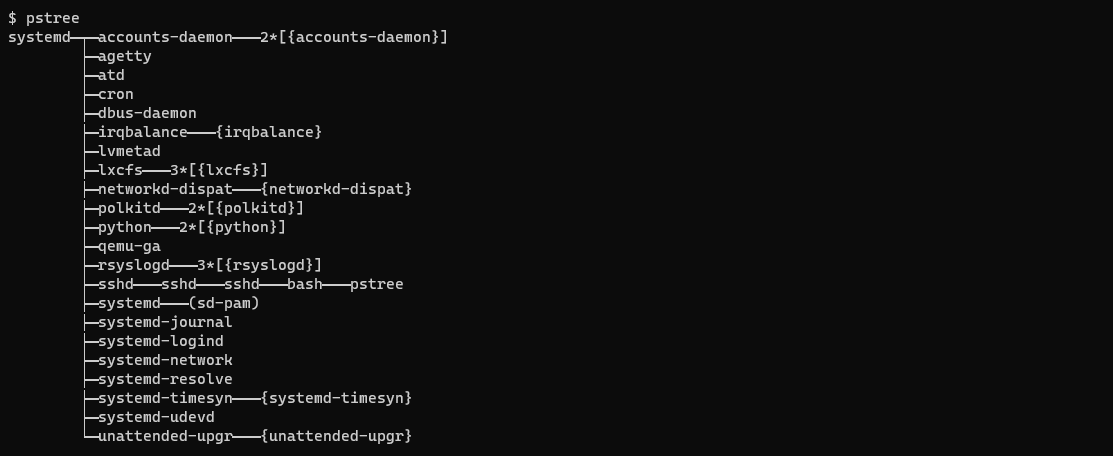
\includegraphics[keepaspectratio]{media/C09_procesos/pstree.png}
\caption{Ejemplo de árbol de procesos mostrador por el comando
pstree.}\label{fig-pstree}
\end{figure}

En estos sistemas se conoce como proceso \textbf{{}init} al proceso
padre raíz de todos los procesos de usuario. Su PID siempre es 1, ya que
es el primer proceso creado por el sistema operativo al terminar la
inicialización del núcleo. Por lo tanto, es el responsable de crear
todos los otros procesos que son necesarios para el funcionamiento del
sistema.

En la \hyperref[fig-pstree]{Ejemplo de árbol de procesos mostrador por
el comando pstree.} se observa que \texttt{systemd} es el proceso
\textbf{{}init}, como ocurre frecuentemente en muchos sistemas Linux
actuales. Anteriormente, lo común es que los sistemas Linux emplearan
una implementación de \textbf{{}init} basada en la de los UNIX System V.

\subsubsection{Cómo obtienen los procesos hijos los recursos que
necesitan}\label{_como_obtienen_los_procesos_hijos_los_recursos_que_necesitan}

Hay varios aspectos en la creación de los procesos que pueden variar de
un sistema operativo a otro. Uno de ellos es cómo obtienen los procesos
hijos los recursos que necesitan para hacer su trabajo.

Fundamentalmente existen dos alternativas:

\begin{enumerate}
\def\labelenumi{\arabic{enumi}.}
\item
  Que cada proceso hijo pueda solicitar y obtener los recursos
  directamente del sistema operativo, compitiendo por los recursos del
  sistema en las mismas condiciones que el resto de procesos en
  ejecución. Esta es la opción más común en los sistemas de propósito
  general actuales, como Microsoft Windows, Android, Linux, macOS, UNIX
  BSD y muchos otros.
\item
  Que los procesos hijo solo puedan aspirar a obtener un subconjunto de
  los recursos de su padre. Esto es interesante en sistemas diseñados
  para ser muy robustos, ya que evita que un proceso pueda sobrecargar
  el sistema creando múltiples procesos que consuman demasiada memoria o
  tiempo de CPU.
\end{enumerate}

En este último caso, el proceso padre puede estar obligado a repartir
sus recursos entre los procesos hijo. O puede que el sistema les permita
compartir algunos de esos recursos ---como memoria o archivos--- con
algunos de sus hijos.

\subsubsection{Cómo pasar parámetros de inicialización a los procesos
hijo}\label{_como_pasar_paruxe1metros_de_inicializacion_a_los_procesos_hijo}

Generalmente, el proceso padre suele disponer de algún mecanismo para
pasar parámetros de inicialización a sus procesos hijo.

\paragraph{Argumentos de línea de
comandos}\label{_argumentos_de_luxednea_de_comandos}

Por ejemplo, en Windows API un proceso puede usar el segundo argumento
de \{win32\_createprocess\} para indicar al proceso hijo opciones y
argumentos de línea de comandos:

\begin{Shaded}
\begin{Highlighting}[]
\NormalTok{HANDLE handle }\OperatorTok{=}\NormalTok{ CreateProcess}\OperatorTok{(}\StringTok{"C:}\SpecialCharTok{\textbackslash{}\textbackslash{}}\StringTok{holamundo.exe"}\OperatorTok{,} \StringTok{"/v /s foo.txt bar.png"}\OperatorTok{,} \CommentTok{/* ... */} \OperatorTok{);}
\end{Highlighting}
\end{Shaded}

Si el proceso hijo está programado en C o C++, podrá acceder a los
argumentos \texttt{/v}, \texttt{/s}, \texttt{foo.txt} y \texttt{bar.png}
a través de los argumentos \texttt{argc} y \texttt{argv} de la función
\{clang\_main\} del programa:

\begin{Shaded}
\begin{Highlighting}[]
\DataTypeTok{int}\NormalTok{ main }\OperatorTok{(}\DataTypeTok{int}\NormalTok{ argc}\OperatorTok{,} \DataTypeTok{char}\OperatorTok{*}\NormalTok{ argv}\OperatorTok{[])}
\OperatorTok{\{}
    \CommentTok{/* . . . */}
\OperatorTok{\}}
\end{Highlighting}
\end{Shaded}

de forma que \texttt{argv{[}0{]}} contendrá \texttt{/v},
\texttt{argv{[}2{]}} contendrá \texttt{/s} y así sucesivamente.

Obviamente, en otros lenguajes de programación se accede de manera
diferente a estos argumentos de línea de comandos.

\paragraph{Variables de entorno}\label{_variables_de_entorno}

Otra forma de pasar parámetros a un proceso hijo es usando las
\textbf{variables de entorno}, que no son sino variables dinámicas que
se pueden crear, leer y modificar durante la ejecución del proceso.

Las \textbf{variables de entorno} se gestionan con funciones específicas
ofrecidas por la API del sistema operativo:

\begin{longtable}[]{@{}
  >{\raggedright\arraybackslash}p{(\linewidth - 4\tabcolsep) * \real{0.3333}}
  >{\raggedright\arraybackslash}p{(\linewidth - 4\tabcolsep) * \real{0.3333}}
  >{\raggedright\arraybackslash}p{(\linewidth - 4\tabcolsep) * \real{0.3333}}@{}}
\caption{Funciones de la API para gestionar variables de
entorno.}\tabularnewline
\toprule\noalign{}
\begin{minipage}[b]{\linewidth}\raggedright
\end{minipage} & \begin{minipage}[b]{\linewidth}\raggedright
POSIX API
\end{minipage} & \begin{minipage}[b]{\linewidth}\raggedright
Windows API
\end{minipage} \\
\midrule\noalign{}
\endfirsthead
\toprule\noalign{}
\begin{minipage}[b]{\linewidth}\raggedright
\end{minipage} & \begin{minipage}[b]{\linewidth}\raggedright
POSIX API
\end{minipage} & \begin{minipage}[b]{\linewidth}\raggedright
Windows API
\end{minipage} \\
\midrule\noalign{}
\endhead
\bottomrule\noalign{}
\endlastfoot
\textbf{Leer} & \{clang\_getenv\} & \{win32\_getenvironmentvariable\} \\
\textbf{Leer todos} & \{clang\_environ\} &
\{win32\_getenvironmentstrings\} \\
\textbf{Crear / modificar} & \{clang\_setenv\} &
\{win32\_setenvironmentvariable\} \\
\end{longtable}

por ejemplo, en sistemas POSIX un programa puede leer la variable de
entorno \texttt{PATH} así:

\begin{Shaded}
\begin{Highlighting}[]
\DataTypeTok{char}\OperatorTok{*}\NormalTok{ path }\OperatorTok{=}\NormalTok{ getenv}\OperatorTok{(}\StringTok{"PATH"}\OperatorTok{);}
\end{Highlighting}
\end{Shaded}

mientras que en Windows API es así:

\begin{Shaded}
\begin{Highlighting}[]
\NormalTok{DWORD buffSize }\OperatorTok{=} \DecValTok{4096}\OperatorTok{;}
\NormalTok{TCHAR path}\OperatorTok{[}\NormalTok{buffSize}\OperatorTok{];}
\NormalTok{GetEnvironmentVariable}\OperatorTok{(}\StringTok{"PATH"}\OperatorTok{,}\NormalTok{ path}\OperatorTok{,}\NormalTok{ buffSize}\OperatorTok{);} 
\end{Highlighting}
\end{Shaded}

\begin{itemize}
\item
  El valor de la variable de entorno \texttt{PATH} se copia en
  \texttt{path}.
\end{itemize}

Usando \{clang\_setenv\} o \{win32\_setenvironmentvariable\} de forma
similar, cualquier proceso puede crear variables de entorno que serán
accesibles a sus procesos hijos, porque por defecto los nuevos procesos
heredan un duplicado de las variables de entorno de su proceso padre.
Así se pueden pasar parámetros de configuración para alterar el
comportamiento de los procesos hijo.

Todas las variantes de sistemas UNIX, así como MS-DOS y todas las
versiones de Microsoft Windows soportan variables de entorno.

\paragraph{Herencia de recursos}\label{_herencia_de_recursos}

En algunos sistemas operativos los procesos hijos pueden heredar cierto
tipo de recursos del proceso padre, lo que también puede servir para
inicializar y alterar el comportamiento del proceso hijo.

Por ejemplo, en los sistemas POSIX todos los archivos abiertos por un
proceso son heredados en el mismo estado por sus hijos. Lo interesante
es que en estos sistemas muchos recursos se gestionan como archivos.
Algunos ejemplos podrían ser: dispositivos de E/S, memoria compartida,
tuberías, \emph{sockets} y otros mecanismos de comunicación.

En POSIX todo proceso tiene, por defecto, tres archivos abiertos que
corresponden a tres dispositivos de E/S especiales:

\begin{itemize}
\item
  \textbf{Entrada estándar}{}, de donde los procesos leen la entrada del
  teclado de la terminal.
\item
  \textbf{Salida estándar}{}, donde el proceso escribe para mostrar
  texto en la pantalla de la terminal.
\item
  \textbf{Salida de error}{}, usada para mostrar errores en la pantalla
  de la terminal.
\end{itemize}

Debido a la herencia de los archivos abiertos del proceso padre, todo
proceso hijo tiene acceso a estos tres mismos dispositivos. Y a su vez
también la tendrán sus hijos y los hijos de estos. De esta manera, todo
proceso tiene acceso a los dispositivos de E/S de la terminal donde se
ejecuta. Pero también permite a un proceso controlar el destino de la
E/S de un proceso hijo ---y de los hijos de este---.

Por ejemplo, si antes de crear el proceso hijo sustituye el dispositivo
de salida estándar por un archivo real, todo lo que el hijo intente
mostrar por pantalla se guardará en dicho archivo, en lugar de
mostrarse. Mientras que si lo hace con el dispositivo de entrada
estándar, todo lo que pretenda leer de teclado realmente lo leerá de un
archivo que el padre puede haber preparado, como si de algún tipo de
control remoto se tratara.

Esta misma idea se puede extender a procesos que ofrecen servicios, ya
sea a otros procesos del mismo sistema o a redes de ordenadores, como
Internet.

Cada conexión con un cliente es como archivo abierto, por lo que los
hijos del proceso heredan las conexiones. Así que es común la estrategia
de crear un hijo por conexión para que la atienda en nombre del padre,
mientras este se encarga de recibir nuevas conexiones.

En Microsoft Windows existe un mecanismo similar pero no por defecto. La
función \{win32\_createprocess\} de Windows API permite indicar si se
quiere que el nuevo proceso herede los recursos abiertos. Y también
tiene ajustes específicos para la entrada y salida estándar y la salida
de error del nuevo proceso.

\subsubsection{Qué ocurre con la ejecución del
padre}\label{_quuxe9_ocurre_con_la_ejecucion_del_padre}

Se suelen contemplar dos posibilidades en términos de la ejecución del
padre:

\begin{enumerate}
\def\labelenumi{\arabic{enumi}.}
\item
  Que el padre continúe ejecutándose al mismo tiempo que el hijo. Es lo
  más común en los sistemas multitarea actuales.
\item
  Que el padre quede detenido a la espera de que algunos o todos sus
  hijos terminen. Era lo más frecuente en sistemas monotarea, como
  \{msdos\}.
\end{enumerate}

\subsubsection{Cómo se construye el espacio de direcciones de los
procesos
hijo}\label{_como_se_construye_el_espacio_de_direcciones_de_los_procesos_hijo}

En general hay dos posibilidades:

\begin{enumerate}
\def\labelenumi{\arabic{enumi}.}
\item
  Que el espacio de direcciones del proceso hijo sea un duplicado del
  que tiene el padre. Es decir, que inicialmente el hijo tenga el mismo
  código y datos que el padre. Es lo que hace \{linux\_fork\} en los
  sistemas POSIX.
\item
  Que el espacio de direcciones del proceso hijo se cree desde cero y se
  cargue en él un nuevo programa. Es lo que hace
  \{win32\_createprocess\} en Windows. Por eso siempre hay que indicarle
  el nombre del programa que se quiere ejecutar en el nuevo proceso.
\end{enumerate}

Esto lo veremos con más detalle en el
\hyperref[_ejemplos_de_operaciones_con_procesos]{Ejemplos de operaciones
con procesos}.

\subsection{Terminación de procesos}\label{_terminacion_de_procesos}

Un proceso termina cuando se lo indica al sistema operativo con la
llamada al sistema \textbf{exit}. En ese momento puede devolver un valor
de estado a su padre.

Esto ocurre en C y C++ incluso si el programa termina usando la
sentencia \texttt{return} en \{clang\_main\}. Lo que ocurre es que es el
código, introducido por el compilador, que llamó a \{clang\_main\} es el
que llama a \textbf{exit} usando el valor devuelto por \{clang\_main\}.

El proceso padre puede esperar a que el hijo termine y recuperar ese
valor a través de la llamada al sistema \textbf{wait}. Cuando un proceso
termina, todos los recursos son liberados, incluyendo: la memoria física
y virtual, archivos y dispositivos abiertos, búferes de E/S, etc.

\begin{longtable}[]{@{}
  >{\raggedright\arraybackslash}p{(\linewidth - 4\tabcolsep) * \real{0.3333}}
  >{\raggedright\arraybackslash}p{(\linewidth - 4\tabcolsep) * \real{0.3333}}
  >{\raggedright\arraybackslash}p{(\linewidth - 4\tabcolsep) * \real{0.3333}}@{}}
\caption{Funciones de la API para salir, esperar y terminar
procesos.}\tabularnewline
\toprule\noalign{}
\begin{minipage}[b]{\linewidth}\raggedright
\end{minipage} & \begin{minipage}[b]{\linewidth}\raggedright
POSIX API
\end{minipage} & \begin{minipage}[b]{\linewidth}\raggedright
Windows API
\end{minipage} \\
\midrule\noalign{}
\endfirsthead
\toprule\noalign{}
\begin{minipage}[b]{\linewidth}\raggedright
\end{minipage} & \begin{minipage}[b]{\linewidth}\raggedright
POSIX API
\end{minipage} & \begin{minipage}[b]{\linewidth}\raggedright
Windows API
\end{minipage} \\
\midrule\noalign{}
\endhead
\bottomrule\noalign{}
\endlastfoot
\textbf{Salir} & \{clang\_exit\} & \{win32\_exitprocess\} \\
\textbf{Esperar (un hijo concreto)} & \{linux\_waitpid\} &
\{win32\_waitforsingleobject\} \\
\textbf{Esperar (múltiples hijos)} & \{linux\_wait\} &
\{win32\_waitformultipleobjects\} \\
\textbf{Terminar otro proceso} & \{linux\_kill\} &
\{win32\_terminateprocess\} \\
\end{longtable}

En todo caso un proceso puede provocar la terminación de otro proceso a
través de una llamada al sistema. Por ejemplo, en sistemas POSIX se usa
un mecanismo llamado \textbf{señales}{}:

\begin{Shaded}
\begin{Highlighting}[]
\NormalTok{kill}\OperatorTok{(}\NormalTok{pid}\OperatorTok{,}\NormalTok{ SIGTERM}\OperatorTok{);}
\end{Highlighting}
\end{Shaded}

mientras que en Windows API:

\begin{Shaded}
\begin{Highlighting}[]
\NormalTok{TerminateProcess}\OperatorTok{(}\NormalTok{handle}\OperatorTok{);}
\end{Highlighting}
\end{Shaded}

Habitualmente el proceso que invoca estas funciones es el proceso padre,
ya que puede que sea el único con permisos para hacerlo.

Los motivos para terminar un proceso hijo pueden ser:

\begin{itemize}
\item
  \textbf{El hijo ha excedido el uso de algunos de los recursos
  reservados}. Obviamente esto tiene sentido cuando los hijos utilizan
  un subconjunto de los recursos asignados al padre.
\item
  \textbf{La tarea asignada al hijo ya no es necesaria}. Por ejemplo, se
  creó para comprimir un archivo, pero el usuario ha pedido cancelar la
  operación.
\item
  \textbf{El padre termina y el sistema operativo está diseñado para no
  permitir que el hijo pueda seguir ejecutándose si no tiene un padre}.
  En esos sistemas, la terminación de un proceso provoca que el sistema
  operativo inicie lo que se denomina una \textbf{{}terminación en
  cascada}, en la que termina todos los procesos que cuelgan de dicho
  proceso.
\end{itemize}

En sistemas UNIX y estilo UNIX, si un proceso muere a sus hijos no
terminan sino que se les reasigna como padre el proceso \textbf{init}.

\subsection{Ejemplos de operaciones con
procesos}\label{_ejemplos_de_operaciones_con_procesos}

En C estándar la función \{clang\_system\} de la librería estándar
permite ejecutar otro proceso, con sus argumentos, esperar a que termine
y obtener el valor de estado con el que finalizó el proceso.

\begin{Shaded}
\begin{Highlighting}[]
\DataTypeTok{int}\NormalTok{ status }\OperatorTok{=}\NormalTok{ system}\OperatorTok{(}\StringTok{"holamundo {-}v foo.txt"}\OperatorTok{);}
\end{Highlighting}
\end{Shaded}

Esta función es portable. Está disponible en cualquier sistema donde
haya un compilador de C estándar, pero sus funcionalidades son bastante
limitadas. Por ejemplo, no permite que el programa padre continúe su
ejecución mientras se ejecuta el hijo, aunque el sistema sea multitarea
y ese sea el comportamiento por defecto. Tampoco facilita el control de
los recursos que son heredados por el proceso hijo o hacer redirecciones
de los dispositivos de E/S estándar.

Como hemos comentado anteriormente, para acceder a todas las
funcionalidades ofrecidas por los sistemas operativos, muchas veces es
necesario utilizar directamente la librería del sistema.

\subsubsection{Windows API}\label{_windows_api}

En Windows la librería del sistema ofrece la función
\{win32\_createprocess\}. A diferencia de \{clang\_system\}, recibe
muchísimos argumentos, ya que permite configurar bastantes aspectos de
la creación de un nuevo proceso.

En el \hyperref[ejemplo-createprocess]{example\_title} se puede ver cómo
se usa \{win32\_createprocess\} para ejecutar un programa y esperar a
que termine, de forma similar a como lo hace \{clang\_system\}.

El código fuente completo de este ejemplo está disponible en
\{createprocess\_cpp\}.

\begin{Shaded}
\begin{Highlighting}[]
\NormalTok{STARTUPINFO si }\OperatorTok{=} \OperatorTok{\{} \KeywordTok{sizeof}\OperatorTok{(}\NormalTok{STARTUPINFO}\OperatorTok{)} \OperatorTok{\};} 
\NormalTok{PROCESS\_INFORMATION pi }\OperatorTok{=} \OperatorTok{\{}\DecValTok{0}\OperatorTok{\};} 

\CommentTok{// Crear procesos hijo y comprobar si no se creó con éxito.}
\ControlFlowTok{if}\OperatorTok{(} \OperatorTok{!}\NormalTok{ CreateProcess}\OperatorTok{(} 
\NormalTok{    NULL}\OperatorTok{,} 
    \StringTok{"C:}\SpecialCharTok{\textbackslash{}\textbackslash{}}\StringTok{Windows}\SpecialCharTok{\textbackslash{}\textbackslash{}}\StringTok{System32}\SpecialCharTok{\textbackslash{}\textbackslash{}}\StringTok{charmap.exe"}\OperatorTok{,}  
\NormalTok{    NULL}\OperatorTok{,}
\NormalTok{    NULL}\OperatorTok{,}
\NormalTok{    FALSE}\OperatorTok{,} 
    \DecValTok{0}\OperatorTok{,}
\NormalTok{    NULL}\OperatorTok{,}  
\NormalTok{    NULL}\OperatorTok{,}  
    \OperatorTok{\&}\NormalTok{si}\OperatorTok{,}
    \OperatorTok{\&}\NormalTok{pi }\OperatorTok{))}
\OperatorTok{\{}
\NormalTok{    fprintf}\OperatorTok{(}\NormalTok{ stderr}\OperatorTok{,} \StringTok{"Error (}\SpecialCharTok{\%d}\StringTok{) al crear el proceso.}\SpecialCharTok{\textbackslash{}n}\StringTok{"}\OperatorTok{,}\NormalTok{ GetLastError}\OperatorTok{()} \OperatorTok{);} 
    \ControlFlowTok{return}\NormalTok{ EXIT\_FAILURE}\OperatorTok{;}
\OperatorTok{\}}

\NormalTok{printf}\OperatorTok{(} \StringTok{"[PADRE] El PID del nuevo proceso hijo es: }\SpecialCharTok{\%d\textbackslash{}n}\StringTok{"}\OperatorTok{,}\NormalTok{ pi}\OperatorTok{.}\NormalTok{dwProcessId }\OperatorTok{);}

\CommentTok{// Esperar hasta que el hijo termine.}
\NormalTok{WaitForSingleObject}\OperatorTok{(}\NormalTok{ pi}\OperatorTok{.}\NormalTok{hProcess}\OperatorTok{,}\NormalTok{ INFINITE }\OperatorTok{);} 

\NormalTok{DWORD dwExitCode}\OperatorTok{;}
\NormalTok{GetExitCodeProcess}\OperatorTok{(}\NormalTok{ pi}\OperatorTok{.}\NormalTok{hProcess}\OperatorTok{,} \OperatorTok{\&}\NormalTok{dwExitCode }\OperatorTok{);} 
\NormalTok{printf}\OperatorTok{(} \StringTok{"[PADRE] El valor de salida del proceso hijo es: }\SpecialCharTok{\%d\textbackslash{}n}\StringTok{"}\OperatorTok{,}\NormalTok{ dwExitCode }\OperatorTok{);}

\CommentTok{// Cerrar los manejadores del proceso y del hilo principal del proceso.}
\NormalTok{CloseHandle}\OperatorTok{(}\NormalTok{ pi}\OperatorTok{.}\NormalTok{hProcess }\OperatorTok{);} 
\NormalTok{CloseHandle}\OperatorTok{(}\NormalTok{ pi}\OperatorTok{.}\NormalTok{hThread }\OperatorTok{);}
\end{Highlighting}
\end{Shaded}

\begin{itemize}
\item
  \{win32\_startupinfo\} sirve para pasar a \{win32\_createprocess\}
  parámetros adicionales sobre el inicio de la aplicación, como
  configurar la redirección de la E/S estándar o características de la
  primera ventana creada por la aplicación ---en aplicaciones con
  interfaz gráfica---. Si no se va a usar, debe inicializarse a 0,
  excepto el primer campo que debe contener el tamaño de la estructura.
\item
  \{win32\_processinformation\} sirve para devolver el manejador y el
  \textbf{identificador de proceso} del nuevo proceso. Es común
  inicializar la estructura a 0.
\item
  \{win32\_createprocess\} devuelve \texttt{TRUE} o \texttt{FALSE}, en
  función de si ha tenido éxito o no, respectivamente.
\item
  El primer argumento ---\texttt{lpApplicationName}--- se usa para pasar
  la ruta del ejecutable, mientras que los argumentos de línea de
  comando generalmente se pasan por el segundo
  ---\texttt{lpCommandLine}---. Si en \texttt{lpApplicationName} se
  indica NULL, se puede pasar todo junto por \texttt{lpCommandLine}.
\item
  En \texttt{lpCommandLine} indicamos la ruta al ejecutable y los
  argumentos de la línea de comandos, si hicieran falta.
\item
  Con \texttt{bInheritHandles} a \texttt{FALSE} señalamos que no
  queremos que el proceso hijo herede ningún manejador abierto del
  proceso padre. Estos manejadores son recursos a los que el padre tiene
  acceso y, si fuera necesario, el hijo también podría tenerlo. Los
  manejadores pueden representar, por ejemplo, archivos abiertos,
  tuberías, \emph{sockets} u otros mecanismos de comunicación, procesos
  o archivos mapeados en memoria, entre muchos otros tipos de recursos.
\item
  Con \texttt{NULL} en \texttt{lpEnvironment} indicamos que el hijo
  herede el conjunto de variables de entorno directamente del padre. La
  otra opción es indicar un nuevo conjunto de variables de entorno.
\item
  \texttt{lpCurrentDirectory} sirve para indicar el directorio del
  trabajo del proceso hijo. Es decir, el directorio respecto al que se
  resolverán las rutas de archivo relativas. Con \texttt{NULL} indicamos
  que utilice la misma ruta que el proceso padre.
\item
  Si \{win32\_createprocess\} falla, devuelve \texttt{FALSE}. Llamando a
  \{win32\_getlasterror\} obtiene el código que identifica el motivo del
  error de la última función utilizada de Windows API.
\item
  Usando \{win32\_waitforsingleobject\} hacemos que el proceso padre se
  quede en estado \textbf{esperando} ---sin que pueda seguir
  ejecutándose--- hasta que el proceso hijo termine.
\item
  Cuando el proceso ha terminado, el padre puede conocer su valor de
  salida. Es decir, el valor usado para terminar en la sentencia
  \texttt{return} de \{clang\_main\} o al llamar a
  \{win32\_exitprocess\} en el programa del proceso hijo. Como
  convención, el hijo indica con un 0 que terminó con éxito, mientras
  que con un valor distinto indica que tuvo algún tipo de problema.
\item
  Cuando ya no hace falta obtener información del proceso hijo o
  manipularlo, es necesario cerrar los manejadores devueltos por
  \{win32\_createprocess\}. Así el sistema operativo sabe que las
  estructuras de datos relacionadas con el proceso hijo ya no son
  necesarias, por lo que pueden liberarse.
\end{itemize}

\{win32\_createprocess\} siempre necesita la ruta a un ejecutable ---sea
en el primer o en el segundo argumento de la función--- porque se
utiliza para crear un proceso completamente limpio y ejecutar en él un
nuevo programa.

\subsubsection{POSIX API}\label{sect-procesos-posix-api}

Por el contrario, en los sistemas POSIX se utiliza una estrategia muy
diferente. Los nuevos procesos se crean con la llamada \{linux\_fork\},
que se encarga de crearlo como una copia del proceso padre.

El código fuente completo de este ejemplo está disponible en
\{fork\_cpp\}.

\begin{Shaded}
\begin{Highlighting}[]
\NormalTok{pid\_t pid }\OperatorTok{=}\NormalTok{ getpid}\OperatorTok{();} 

\CommentTok{// Crear un proceso hijo}
\NormalTok{pid\_t child }\OperatorTok{=}\NormalTok{ fork}\OperatorTok{();} 

\ControlFlowTok{if} \OperatorTok{(}\NormalTok{child }\OperatorTok{==} \DecValTok{0}\OperatorTok{)} 
\OperatorTok{\{}
    \CommentTok{// Aquí solo entra el proceso hijo}
\NormalTok{    puts}\OperatorTok{(} \StringTok{"[HIJO] ¡Soy el proceso hijo!"} \OperatorTok{);}
\NormalTok{    printf}\OperatorTok{(} \StringTok{"[HIJO] El valor de mi variable \textquotesingle{}child\textquotesingle{} es: }\SpecialCharTok{\%d\textbackslash{}n}\StringTok{"}\OperatorTok{,}\NormalTok{ child }\OperatorTok{);} 
\NormalTok{    printf}\OperatorTok{(} \StringTok{"[HIJO] Este es mi PID: }\SpecialCharTok{\%d\textbackslash{}n}\StringTok{"}\OperatorTok{,}\NormalTok{ getpid}\OperatorTok{()} \OperatorTok{);} 
\NormalTok{    printf}\OperatorTok{(} \StringTok{"[HIJO] El valor de mi variable \textquotesingle{}pid\textquotesingle{} es: }\SpecialCharTok{\%d\textbackslash{}n}\StringTok{"}\OperatorTok{,}\NormalTok{ pid }\OperatorTok{);} 
\NormalTok{    printf}\OperatorTok{(} \StringTok{"[HIJO] El PID de mi padre es: }\SpecialCharTok{\%d\textbackslash{}n}\StringTok{"}\OperatorTok{,}\NormalTok{ getppid}\OperatorTok{()} \OperatorTok{);} 

\NormalTok{    puts}\OperatorTok{(} \StringTok{"[HIJO] Durmiendo 10 segundos..."} \OperatorTok{);}
\NormalTok{    sleep}\OperatorTok{(}\DecValTok{10}\OperatorTok{);}

    \DataTypeTok{int}\NormalTok{ status }\OperatorTok{=} \DecValTok{42}\OperatorTok{;}
\NormalTok{    printf}\OperatorTok{(} \StringTok{"[HIJO] Salgo con }\SpecialCharTok{\%d}\StringTok{ ¡Adios!}\SpecialCharTok{\textbackslash{}n}\StringTok{"}\OperatorTok{,}\NormalTok{ status }\OperatorTok{);}
    \ControlFlowTok{return}\NormalTok{ status}\OperatorTok{;} 
\OperatorTok{\}}
\ControlFlowTok{else} \ControlFlowTok{if} \OperatorTok{(}\NormalTok{child }\OperatorTok{\textgreater{}} \DecValTok{0}\OperatorTok{)}  
\OperatorTok{\{}
    \CommentTok{// Aquí solo entra el proceso padre}
\NormalTok{    puts}\OperatorTok{(} \StringTok{"[PADRE] ¡Soy el proceso padre!"} \OperatorTok{);}
\NormalTok{    printf}\OperatorTok{(} \StringTok{"[PADRE] El valor de mi variable \textquotesingle{}child\textquotesingle{} es: }\SpecialCharTok{\%d\textbackslash{}n}\StringTok{"}\OperatorTok{,}\NormalTok{ child }\OperatorTok{);}  
\NormalTok{    printf}\OperatorTok{(} \StringTok{"[PADRE] Este es mi PID: }\SpecialCharTok{\%d\textbackslash{}n}\StringTok{"}\OperatorTok{,}\NormalTok{ getpid}\OperatorTok{()} \OperatorTok{);} 
\NormalTok{    printf}\OperatorTok{(} \StringTok{"[PADRE] El valor de mi variable \textquotesingle{}pid\textquotesingle{} es: }\SpecialCharTok{\%d\textbackslash{}n}\StringTok{"}\OperatorTok{,}\NormalTok{ pid }\OperatorTok{);} 
\NormalTok{    printf}\OperatorTok{(} \StringTok{"[PADRE] El PID de mi padre es: }\SpecialCharTok{\%d\textbackslash{}n}\StringTok{"}\OperatorTok{,}\NormalTok{ getppid}\OperatorTok{()} \OperatorTok{);}

\NormalTok{    puts}\OperatorTok{(} \StringTok{"[PADRE] Voy a esperar a que mi hijo termine..."} \OperatorTok{);}

    \DataTypeTok{int}\NormalTok{ status}\OperatorTok{;}
\NormalTok{    wait}\OperatorTok{(} \OperatorTok{\&}\NormalTok{status }\OperatorTok{);}  
\NormalTok{    printf}\OperatorTok{(} \StringTok{"[PADRE] El valor de salida de mi hijo fue: }\SpecialCharTok{\%d\textbackslash{}n}\StringTok{"}\OperatorTok{,}
\NormalTok{        WEXITSTATUS}\OperatorTok{(}\NormalTok{status}\OperatorTok{)} \OperatorTok{);} 

\NormalTok{    puts}\OperatorTok{(} \StringTok{"[PADRE] ¡Adios!"} \OperatorTok{);}
    \ControlFlowTok{return}\NormalTok{ EXIT\_SUCCESS}\OperatorTok{;}
\OperatorTok{\}}
\ControlFlowTok{else} \OperatorTok{\{} 
    \CommentTok{// Aquí solo entra el padre si no pudo crear el hijo}
\NormalTok{    fprintf}\OperatorTok{(}\NormalTok{ stderr}\OperatorTok{,} \StringTok{"Error (}\SpecialCharTok{\%d}\StringTok{) al crear el proceso: }\SpecialCharTok{\%s\textbackslash{}n}\StringTok{"}\OperatorTok{,}
\NormalTok{        errno}\OperatorTok{,}\NormalTok{ strerror}\OperatorTok{(}\NormalTok{errno}\OperatorTok{)} \OperatorTok{);} 
    \ControlFlowTok{return}\NormalTok{ EXIT\_FAILURE}\OperatorTok{;}
\OperatorTok{\}}
\end{Highlighting}
\end{Shaded}

\begin{itemize}
\item
  El proceso llama a \{linux\_fork\} pero al retornar de la llamada
  vuelven dos procesos: el proceso padre, que es el que llamó
  originalmente a \{linux\_fork\}, y el proceso hijo. Como el proceso
  hijo es una copia del padre, tiene el mismo código, las mismas
  variables y los mismos recursos que tenía el padre en el momento de
  llamar a \{linux\_fork\}. La única diferencia es el valor devuelto por
  \{linux\_fork\}, que guardamos en \texttt{child}.
\item
  Los dos procesos ejecutan el mismo programa, así que ambos llegan a la
  línea detrás del \{linux\_fork\}. Como queremos que cada proceso haga
  cosas diferentes, necesitamos que cada uno vaya a ramas distintas del
  código. Eso se hace comprobando el valor de \texttt{child}, porque si
  vale 0 es que el proceso que actualmente ejecuta el programa es el
  hijo.
\item
  Si, por el contrario, el valor de \texttt{child} es mayor de 0, el
  proceso que ejecuta el programa es el padre y el valor de
  \texttt{child} es el PID del proceso hijo creado.
\item
  Así que el valor de \texttt{child} en el padre coincide con el
  devuelto por \{linux\_getpid\} en el hijo.
\item
  Finalmente, si el valor devuelto por \{linux\_fork\} es negativo, es
  que ocurrió un error y el proceso hijo no llegó a crearse.
\item
  En los sistemas POSIX es común que las llamadas al sistema devuelvan
  un valor negativo para indicar un error. El motivo del error se puede
  conocer a través de la variable global \{linux\_errno\}, que siempre
  guarda el código de identificación del error en la última función
  invocada de la API POSIX. La función \{linux\_strerror\} permite
  obtener un texto descriptivo de cualquier valor de \{linux\_errno\},
  lo que siempre resulta útil para crear mensajes de error que ayuden a
  determinar dónde estuvo el problema.
\item
  A modo de ejemplo hemos guardado el PID del proceso en la variable
  \texttt{pid}, antes de la llamada a \{linux\_fork\}. Como el proceso
  hijo es una copia del proceso padre, la variable existe en ambos, pero
  en el proceso hijo su valor coincide con lo devuelto por
  \{linux\_getppid\} mientras que en el proceso padre con lo devuelto
  por \{linux\_getpid\}.
\item
  \{linux\_wait\} hace que el proceso padre interrumpa su ejecución
  hasta que algún hijo termine y devuelve el estado de salida en
  \texttt{status}.

  Debemos asegurarnos de llamar a \{linux\_wait\} o \{linux\_waitpid\}
  una vez por cada proceso hijo, en algún momento, porque así es como el
  sistema sabe que el padre ya no tiene más interés en el proceso y
  puede liberar su PCB, donde se guarda el estado de salida. No hacerlo
  genera \textbf{procesos zombi}{} o \emph{defunct}.
\item
  El valor de salida del proceso hijo lo obtiene el proceso padre a
  través del estado de salida devuelto por \{linux\_wait\}. Pero ese
  estado contiene más información sobre la causa por la que el proceso
  terminó. Para recuperar el valor de salida se usa la macro
  \texttt{WEXITSTATUS} sobre el estado de salida.
\end{itemize}

Lo siguiente es un posible resultado de ejecutar el programa anterior en
una terminal de Linux, numerado con las anotaciones realizadas al
código:

\begin{verbatim}
$ ./fork
[PADRE] ¡Soy el proceso padre!
[PADRE] El valor de mi variable 'child' es: 2360 
[PADRE] Este es mi PID: 2359 
[PADRE] El valor de mi variable 'pid' es: 2359 
[HIJO] ¡Soy el proceso hijo!
[PADRE] El PID de mi padre es: 1857
[PADRE] Voy a esperar a que mi hijo termine...
[HIJO] El valor de mi variable 'child' es: 0 
[HIJO] Este es mi PID: 2360
[HIJO] El valor de mi variable 'pid' es: 2359 
[HIJO] El PID de mi padre es: 2359 
[HIJO] Durmiendo 10 segundos...
[HIJO] Salgo con 42 ¡Adios! 
[PADRE] El valor de salida de mi hijo fue: 42 
[PADRE] ¡Adios!
\end{verbatim}

Aunque pueda parecer algo complejo, esta estrategia facilita la
comunicación entre procesos. Es muy sencillo lanzar otro proceso para
hacer una tarea en paralelo que tendrá automáticamente una copia de los
datos del proceso original.

Como se trata de una copia, las nuevas variables o la modificación de
variables existentes que realice cualquiera de los procesos, no serán
visibles para el otro. Es decir, después del \{linux\_fork\} ambos
procesos son completamente independientes. Pero como el proceso hijo
hereda el acceso a todo tipo de recursos abiertos por el proceso padre,
como: archivos, tuberías, \emph{sockets} o regiones de memoria
compartida, entre muchos otros recursos; es muy sencillo crear un canal
de comunicación entre ambos procesos, si fuera necesario.

Sin embargo, \{linux\_fork\} no proporciona una funcionalidad similar a
la de \{clang\_system\}. No sirve para crear otro proceso con un
programa diferente. Para eso necesitamos \{linux\_exec\}, una familia de
funciones cuyo propósito es cargar un nuevo programa en el proceso que
la invoca.

El código fuente completo de este ejemplo está disponible en
\{fork\_exec\_cpp\}.

\begin{Shaded}
\begin{Highlighting}[]
\CommentTok{// Crear un proceso hijo}
\NormalTok{pid\_t child }\OperatorTok{=}\NormalTok{ fork}\OperatorTok{();} 

\ControlFlowTok{if} \OperatorTok{(}\NormalTok{child }\OperatorTok{==} \DecValTok{0}\OperatorTok{)}
\OperatorTok{\{}
    \CommentTok{// Aquí solo entra el proceso hijo}
\NormalTok{    puts}\OperatorTok{(} \StringTok{"[HIJO] ¡Soy el proceso hijo!"} \OperatorTok{);}
\NormalTok{    puts}\OperatorTok{(} \StringTok{"[HIJO] Voy a ejecutar el comando \textquotesingle{}ls\textquotesingle{}"} \OperatorTok{);}

    \CommentTok{/* Hacer otras cosas necesarias antes de ejecutar el programa... */} 

\NormalTok{    execl}\OperatorTok{(} \StringTok{"/bin/ls"}\OperatorTok{,} \StringTok{"ls"}\OperatorTok{,} \StringTok{"{-}l"}\OperatorTok{,}\NormalTok{ NULL }\OperatorTok{);}   

\NormalTok{    fprintf}\OperatorTok{(}\NormalTok{ stderr}\OperatorTok{,} \StringTok{"Error (}\SpecialCharTok{\%d}\StringTok{) al ejecutar el programa: }\SpecialCharTok{\%s\textbackslash{}n}\StringTok{"}\OperatorTok{,}
\NormalTok{        errno}\OperatorTok{,}\NormalTok{ strerror}\OperatorTok{(}\NormalTok{errno}\OperatorTok{)} \OperatorTok{);} 
    \ControlFlowTok{return}\NormalTok{ EXIT\_FAILURE}\OperatorTok{;} 
\OperatorTok{\}}
\ControlFlowTok{else} \ControlFlowTok{if} \OperatorTok{(}\NormalTok{child }\OperatorTok{\textgreater{}} \DecValTok{0}\OperatorTok{)}
\OperatorTok{\{}
    \CommentTok{// Aquí solo entra el proceso padre}
\NormalTok{    puts}\OperatorTok{(} \StringTok{"[PADRE] ¡Soy el proceso padre!"} \OperatorTok{);}
\NormalTok{    puts}\OperatorTok{(} \StringTok{"[PADRE] Voy a esperar a que mi hijo termine..."} \OperatorTok{);}

    \DataTypeTok{int}\NormalTok{ status}\OperatorTok{;}
\NormalTok{    wait}\OperatorTok{(} \OperatorTok{\&}\NormalTok{status }\OperatorTok{);} 
\NormalTok{    printf}\OperatorTok{(} \StringTok{"[PADRE] El valor de salida de mi hijo fue: }\SpecialCharTok{\%d\textbackslash{}n}\StringTok{"}\OperatorTok{,}
\NormalTok{        WEXITSTATUS}\OperatorTok{(}\NormalTok{status}\OperatorTok{)} \OperatorTok{);}

\NormalTok{    puts}\OperatorTok{(} \StringTok{"[PADRE] ¡Adios!"} \OperatorTok{);}
    \ControlFlowTok{return}\NormalTok{ EXIT\_SUCCESS}\OperatorTok{;}
\OperatorTok{\}}
\ControlFlowTok{else} \OperatorTok{\{}
    \CommentTok{// Aquí solo entra el padre si no pudo crear el hijo}
\NormalTok{    fprintf}\OperatorTok{(}\NormalTok{ stderr}\OperatorTok{,} \StringTok{"Error (}\SpecialCharTok{\%d}\StringTok{) al crear el proceso: }\SpecialCharTok{\%s\textbackslash{}n}\StringTok{"}\OperatorTok{,}
\NormalTok{        errno}\OperatorTok{,}\NormalTok{ strerror}\OperatorTok{(}\NormalTok{errno}\OperatorTok{)} \OperatorTok{);}
    \ControlFlowTok{return}\NormalTok{ EXIT\_FAILURE}\OperatorTok{;}
\OperatorTok{\}}
\end{Highlighting}
\end{Shaded}

\begin{itemize}
\item
  Primero creamos un proceso hijo, donde ejecutaremos el nuevo programa.
  Si nos diera por llamar directamente a una función de la familia
  \{linux\_exec\}, nuestro programa sería sustituido y no tendríamos
  ningún control sobre lo que pase después.
\item
  En la rama de código que se va a ejecutar en el hijo ---gracias a la
  comprobación del valor devuelto por \{linux\_fork\}--- ejecutamos la
  función de la familia \{linux\_exec\} que más nos interese. Esta
  función no crea otro proceso, sino que carga el programa indicado en
  el proceso hijo, sustituyendo así a nuestro programa.
\item
  Todas las funciones de la familia \{linux\_exec\} reciben como primer
  argumento la ruta al ejecutable, pero en \texttt{execlp()} en
  particular, a continuación se indican los argumentos de línea de
  comandos, tal y como queremos que los reciba el programa en el
  argumento \texttt{argv} de su \{clang\_main\}. Es decir, que el
  programa del comando \texttt{/bin/ls} recibirá \texttt{ls} y
  \texttt{-l} en \texttt{argv{[}0{]}} y \texttt{argv{[}1{]}},
  respectivamente. El \texttt{NULL} del final indica cuando no hay más
  argumentos de línea de comandos para pasar.
\item
  Antes de ejecutar la función \{linux\_exec\} se pueden hacer cosas
  para configurar adecuadamente el proceso donde se ejecutará el nuevo
  programa. Por ejemplo, cambiar las variables de entorno, redirigir la
  E/S estándar, cambiar el usuario al que pertenece el proceso ---si
  originalmente se ejecuta con un usuario con ese privilegio--- o cerrar
  archivos abiertos del proceso padre que ha heredado el proceso hijo y
  que, obviamente, no queremos que se queden abiertos para programas
  diferentes al nuestro.
\item
  Las funciones \{linux\_exec\} no retornan si tienen éxito, porque el
  programa actual es sustituido por el indicado, que comenzará a
  ejecutarse de su \{clang\_main\}.
\item
  Si la función \{linux\_exec\} retorna es porque falló y, como es
  común, el motivo del error está disponible en \{linux\_errno\}. Un
  motivo de fallo muy típico es que el ejecutable indicado no exista.
\item
  Si la función \{linux\_exec\} retorna, la ejecución del programa en el
  proceso hijo continúa hasta salir de \{clang\_main\}. Generalmente, el
  proceso hijo no es útil si no puede ejecutar el programa que le hemos
  indicado. Por eso es importante asegurarnos de que el proceso hijo
  termina, si \{linux\_exec\} falla.
\item
  Mientras todo lo anterior ocurre en el proceso hijo, el proceso padre
  espera. Cuando el proceso hijo termine, el padre podrá obtener su
  estado de salir para saber si tuvo éxito o no.
\end{itemize}

Lo siguiente es un posible resultado de ejecutar el programa anterior en
una terminal de Linux, numerado con las anotaciones realizadas al
código:

\begin{verbatim}
$ ./fork-exec
[PADRE] ¡Soy el proceso padre!
[PADRE] Voy a esperar a que mi hijo termine...
[HIJO] ¡Soy el proceso hijo!
[HIJO] Voy a ejecutar el comando 'ls'
total 628 
-rwxr--r-- 1 jesus jesus 72640 Sep 16 13:41 fifo-client
-rwxr--r-- 1 jesus jesus 72784 Sep 16 13:41 fifo-server
-rwxr--r-- 1 jesus jesus 20056 Sep 16 13:41 fork
-rwxr-xr-x 1 jesus jesus 19896 Sep 18 13:24 fork-exec
-rwxr--r-- 1 jesus jesus 80744 Sep 16 13:41 mmap
-rwxr--r-- 1 jesus jesus 45712 Sep 16 13:41 pipe
-rwxr--r-- 1 jesus jesus 87024 Sep 16 13:41 shared-memory
-rwxr--r-- 1 jesus jesus 77696 Sep 16 13:41 shared-memory-sync
-rwxr--r-- 1 jesus jesus 19608 Sep 16 13:41 softstack-c
-rwxr--r-- 1 jesus jesus 39328 Sep 16 13:41 softstack-cpp
-rwxr--r-- 1 jesus jesus  9920 Sep 16 13:41 syscall
-rwxr--r-- 1 jesus jesus 40712 Sep 16 13:41 threads-mutex-pthread
-rwxr--r-- 1 jesus jesus 39944 Sep 16 13:41 threads-pthread
[PADRE] El valor de salida de mi hijo fue: 0 
[PADRE] ¡Adios!
\end{verbatim}

Veamos qué ocurre si la línea de la función \{linux\_exec\} fuera:

\begin{Shaded}
\begin{Highlighting}[]
\NormalTok{execl}\OperatorTok{(} \StringTok{"/bin/ls"}\OperatorTok{,} \StringTok{"ls"}\OperatorTok{,} \StringTok{"{-}l"}\OperatorTok{,} \StringTok{"/foo"}\OperatorTok{,}\NormalTok{ NULL }\OperatorTok{);}
\end{Highlighting}
\end{Shaded}

para intentar ver el contenido del directorio \texttt{/foo}, que no
existe:

\begin{verbatim}
$ ./fork-exec
[PADRE] ¡Soy el proceso padre!
[PADRE] Voy a esperar a que mi hijo termine...
[HIJO] ¡Soy el proceso hijo!
[HIJO] Voy a ejecutar el comando 'ls'
ls: cannot access '/foo': No such file or directory 
[PADRE] El valor de salida de mi hijo fue: 2 
[PADRE] ¡Adios!
\end{verbatim}

\begin{itemize}
\item
  El comando \texttt{ls} se ejecuta, pero falla porque el directorio
  indicado no existe.
\item
  Por eso el programa, al terminar el proceso, no devuelve 0 si no 2 y
  es ese el valor que recibe el proceso padre. Esto le permite saber al
  proceso padre que el comando \texttt{ls} no tuvo éxito.
\end{itemize}

Y finalmente cambiemos la línea de la función \{linux\_exec\} así:

\begin{Shaded}
\begin{Highlighting}[]
\NormalTok{execl}\OperatorTok{(} \StringTok{"/noexists"}\OperatorTok{,} \StringTok{"ls"}\OperatorTok{,} \StringTok{"{-}l"}\OperatorTok{,}\NormalTok{ NULL }\OperatorTok{);}
\end{Highlighting}
\end{Shaded}

para que intente ejecutar un programa que no existe:

\begin{verbatim}
$ ./fork-exec
[PADRE] ¡Soy el proceso padre!
[PADRE] Voy a esperar a que mi hijo termine...
[HIJO] ¡Soy el proceso hijo!
[HIJO] Voy a ejecutar el comando 'ls'
Error (2) al ejecutar el programa: No such file or directory 
[PADRE] El valor de salida de mi hijo fue: 255 
[PADRE] ¡Adios!
\end{verbatim}

\begin{itemize}
\item
  \{linux\_exec\} falla y se muestra el mensaje de error con el motivo.
\item
  El proceso hijo termina con -1 y así llega ese valor al proceso padre.
  Al utilizar un valor de salida diferente a los que usa el programa que
  intenta ejecutar, el padre distingue las terminaciones causadas por
  errores al llamar a \{linux\_exec\} de los errores del propio
  programa.
\end{itemize}

Todas las funciones \{linux\_exec\} hacen lo mismo. Primero liberan la
memoria reservada en el proceso, después cargan el nuevo programa y
finalmente inicia la ejecución del programa desde su punto de entrada.
La diferencia entre las distintas funciones está en los argumentos que
aceptan. Esa diferencia se puede conocer fijándonos en las letras al
final del nombre de cada función:

\begin{itemize}
\item
  \textbf{Sin \textquotesingle p\textquotesingle{}}, como
  \texttt{execl()} o \texttt{execv()}, el primer argumento de la función
  es la ruta hasta el ejecutable del programa que se quiere ejecutar.
\item
  \textbf{Con \textquotesingle p\textquotesingle{}}, como
  \texttt{execlp()} o \texttt{execvp()}, la función busca el ejecutable
  como lo hace la \emph{shell}. Es decir, si el primer argumento no
  contiene ninguna \textquotesingle/\textquotesingle{} se toma como el
  nombre del ejecutable y se busca en los directorios listados en la
  variable de entorno \texttt{PATH}. Si el primer argumento contiene
  alguna \textquotesingle/\textquotesingle, se considera una ruta y se
  busca directamente el ejecutable en ella.
\item
  \textbf{Con \textquotesingle l\textquotesingle{}}, como
  \texttt{execl()} o \texttt{execlp()}, los argumentos de línea de
  comandos para pasar al programa se indican directamente como
  argumentos diferentes de la función ---por ejemplo
  \texttt{execl("/bin/ls",\ "ls",\ "-l",\ "-a"\ NULL)}--- lo que es
  ideal cuando el número de argumentos es fijo. La lista de argumentos
  debe terminar en \texttt{NULL}.
\item
  \textbf{Con \textquotesingle v\textquotesingle{}}, como
  \texttt{execv()} o \texttt{execvp()}, los argumentos de la línea de
  comandos para pasar al programa se indican en un \emph{array} de
  punteros a cadenas terminadas en
  \textquotesingle\textbackslash0\textquotesingle, lo que resulta muy
  práctico si el número de argumentos es desconocido en el momento de
  compilar. El último elemento del \emph{array} debe apuntar a
  \texttt{NULL}. Por ejemplo:

\begin{Shaded}
\begin{Highlighting}[]
\DataTypeTok{char}\OperatorTok{*}\NormalTok{ argv}\OperatorTok{[]} \OperatorTok{=} \OperatorTok{\{} \StringTok{"ls"}\OperatorTok{,} \StringTok{"{-}l"}\OperatorTok{,} \StringTok{"{-}a"}\OperatorTok{,}\NormalTok{ NULL }\OperatorTok{\};}
\NormalTok{execv}\OperatorTok{(}\StringTok{"/bin/ls"}\OperatorTok{,}\NormalTok{ argv}\OperatorTok{);}
\end{Highlighting}
\end{Shaded}
\item
  \textbf{Con \textquotesingle e\textquotesingle{}}, como
  \texttt{execvpe()} o \texttt{execle()}, la función admite un argumento
  adicional para indicar el conjunto de variables de entorno con el que
  se ejecutará el nuevo programa. Con las otras funciones
  \{linux\_exec\} se conservan las variables de entorno actuales en el
  proceso que llama a la función.
\end{itemize}

\section{Procesos cooperativos}\label{_procesos_cooperativos}

Desde el punto de vista de la cooperación podemos clasificar los
procesos en dos grupos:

\begin{itemize}
\item
  Los \textbf{procesos independientes}{}, que no afectan o pueden ser
  afectados por otros procesos del sistema. Cualquier proceso que no
  comparte datos ---temporales o persistentes--- con otros procesos es
  independiente.
\item
  Los \textbf{procesos cooperativos}{}, que pueden afectar o ser
  afectados por otros procesos ejecutados en el sistema. Los procesos
  que comparten datos, sea cual sea la forma en la que lo hacen, siempre
  son cooperativos.
\end{itemize}

\subsection{Motivaciones para la colaboración entre
procesos}\label{_motivaciones_para_la_colaboracion_entre_procesos}

Hay diversos motivos para proporcionar un entorno que permita la
cooperación de los procesos:

\begin{itemize}
\item
  \textbf{Compartición de información}. Dado que varios usuarios pueden
  estar interesados en los mismos bloques de información ---por ejemplo,
  en un archivo compartido--- el sistema operativo debe proporcionar un
  entorno que permita el acceso concurrente a este tipo de recursos.
\item
  \textbf{Velocidad de cómputo}. Para que una tarea se ejecute más
  rápido se puede partir en subtareas que se ejecuten en paralelo. Es
  importante destacar que la mejora en la velocidad solo es posible si
  el sistema tiene varios componentes de procesamiento como procesadores
  ---si se quiere acelerar la ejecución en la CPU--- o canales E/S ---si
  se quieren acelerar las operaciones de E/S ---.
\item
  \textbf{Modularidad}. Podemos querer crear nuestro software de forma
  modular, dividiendo las funciones del programa en procesos separados
  que se comunican entre sí.
\item
  \textbf{Conveniencia}. Incluso un usuario individual puede querer
  hacer varias tareas al mismo tiempo. Por ejemplo, editar, imprimir y
  compilar al mismo tiempo.
\end{itemize}

La ejecución simultánea de procesos cooperativos requiere mecanismos
tanto para comunicar unos con otros como para sincronizar sus acciones
(véase el \hyperref[sincronizacion]{???}).

\subsection{Comunicación entre
procesos}\label{_comunicacion_entre_procesos}

Para comunicar procesos cooperativos existen diversas aproximaciones,
que en general se pueden encajar en alguna de las siguientes
estrategias:

\begin{description}
\item[Memoria compartida]
Método de comunicación en el que los procesos utilizan regiones
compartidas de la memoria principal para compartir información.
\item[Paso de mensajes]
Método en el que los procesos utilizan funciones del sistema operativo
para enviarse mensajes entre ellos, compartiendo información y
sincronizando acciones, sin necesidad de compartir memoria.
\end{description}

En la \hyperref[fig-modelos-de-comunicacion]{Modelos de
comunicación.} se puede un esquema comparativo entre ambos modelos de
comunicación. Veremos cada uno en detalle en el
\hyperref[memoria_compartida]{???} y el
\hyperref[comunicacion_mediante_paso_de_mensajes]{???},
respectivamente.

\begin{figure}
\centering
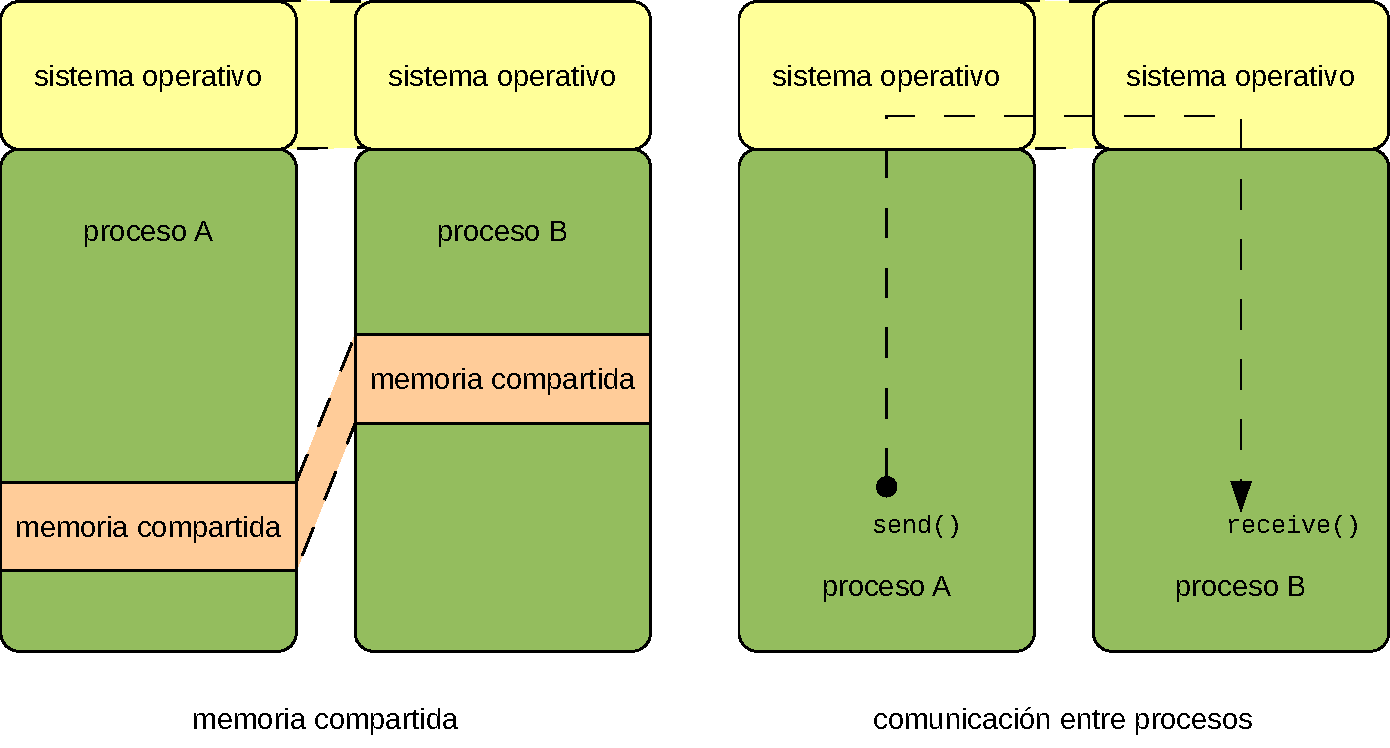
\includegraphics[width=0.8\textwidth]{media/C09_procesos/modelos_comunicación.pdf}
\caption{Modelos de comunicación.}\label{fig-modelos-de-comunicacion}
\end{figure}
